\documentclass[twoside,openright]{wfaiis}
\usepackage{polski}
\usepackage{listings}
\linespread{1.3}
\usepackage{tikz}
\usepackage{amssymb}
\usepackage[?]{amsmath}
\usetikzlibrary{positioning}
\usetikzlibrary{snakes}
\usepackage[utf8]{inputenc}
\usepackage{graphicx}
\usepackage{url}
\usepackage{float}

\autor{Łukasz Stanisławski\album{200617} }
\tytul{Symulacja ciała miękkiego z wykorzystaniem technologii CUDA}
\kierunek{informatyka stosowana}
\zaklad{Katedra Informatyki Stosowanej}
\rodzajpracy{inżynierska}
\promotor{dr hab. Jacek Matulewski}
\jednostkapromotora{Zakład Mechaniki Kwantowej}
\rok{2014}

\lstset{language=C,tabsize=2,basicstyle=\small}

\begin{document}

\maketitle

\tableofcontents

\chapter{Wst�p} %rozpocz�cie pracy nowym rozdzia�em


\chapter{Ciało miękkie w symulacji komputerowej}

\section{Kategoryzacja symulacji}

Publikacje naukowe w dziedzinie symulacji ciał miękkich często mają charakter
iteracyjny. Po stworzeniu nowej metody powstają jej modyfikacje, inni badacze
poprawiają jej parametry, upraszczają,
uszczegóławiają lub nawet łączą ją z innymi znanymi technikami tworząc w ten
sposób nowe rozwiązania. W połączeniu z bardzo dynamicznym rozwojem technologii 
skutkuje to wypieraniem pewnych metod przez inne, lepiej dopasowane do obecnego
stanu wiedzy i sprzętu komputerowego.

Mnogość zastosowań symulacji ciał miękkich sprawiła też, że tematyką tą
zainteresowali są badacze z różnych dziedzin. W efekcie tego obszar modelowania ciał
deformowalnych nabrał prawdziwie interdyscyplinarnego charakteru i łączy dzisiaj w sobie
takie obszary naukowe jak dynamika newtonowska, mechanika ośrodków ciągłych,
metody numeryczne, geometria różniczkowa czy metody aproksymacji\cite{pbdo}.

Bardzo zmienne środowisko, relatywnie młody wiek dziedziny czy jej 
interdyscyplinarny charakter sprawia
że obszar wiedzy na temat komputerowej symulacji ciał deformowalnych relatywnie
trudno opisać.
Jak dotąd znane są mi tylko dwie próby usystematyzowania osiągnięć
tej dziedzinie podjęte w przeciągu ostatnich 30 lat, odnoszące się wyłącznie do
ciał miękkich.

\subsection{Metody fizyczne i niefizyczne}

Pierwszą próbę sklasyfikowania znanych metod symulacji ciał miękkich
podjęli w swoim opracowaniu z 1997 r. Sarah oraz Gibson \cite{TR97-19}. Podzielili
oni wszystkie znane modele na dwie ogólne kategorie: fizyczne oraz niefizyczne. Metody fizyczne, czyli
takie które uwzględniają w swojej budowie pewne prawa fizyczne będą przedmiotem
wnikliwszej analizy w tej pracy. Do modeli niefizycznych zaliczyć można natomiast
krzywe parametryczne oparte na krzywych Breziera czy deformacje brył sztywnych (Free-Form Deformations).\cite{pbdo}

Metody niefizyczne znajdują zastosowanie w obszarach, w których właściwości
fizyczne czy też symulacja zmian obiektu w czasie nie jest celowa. Przykładem
takiego obszaru jest projektowanie komputerowe w programach typu CAD, gdzie
projektowany obiekt musi być przekształcony ze stanu A do B zachowując określone
własności. Nie dziwi zatem fakt, że wszystkie metody niefizyczne są także 
nazywane technikami geometrycznymi.

Do kategorii modeli fizycznych Sarah i Gibson zaliczyli następujące klasy modeli:
\begin{itemize}
\item System Sprężyn (Mass-Spring System)
\item Metody ciągłe (Continuum Models)
\end{itemize}

System sprężyn będzie przedmiotem wnikliwszej analizy w dalszej części tego
rozdziału. W tym miejscu należy jednak określić zakres stosowalności tego
modelu, który obejmuje głównie grafikę komputerową oraz szeroko rozumianą
inżynierię biomedyczną. System sprężyn ze względu na swoje właściwości 
często jest wykorzystywany do symulacji tkanek ciała, gdyż pozwala łatwo łączyć ze
sobą ośrodki o potencjalnie różnych własnościach fizycznych. Dodatkowo symulacje
systemu sprężyn nie są kosztowne obliczeniowo, co pozwala na stosowanie ich w
interaktywnych aplikacjach.

Druga wymieniona w artykule \textit{Survey of Deformable Modelling in Computer Graphics}
klasa modeli wywodzi się z mechaniki ośrodków
ciągłych. Oznacza to, że symulowany obiekt przedstawiany jest jako ciągły
fragment przestrzeni (tzw. continuum) i wykorzystuje równania różniczkowe do
opisania deformacji obiektu. Metody te znajdują zastosowanie w symulacjach
tkanek czy analizie obrazów.\cite{TR97-19}

Metody bazujące na modelu continuum są bardziej fizycznie poprawne niż model
systemu sprężyn\cite{TR97-19}, jednak posiadają pewne niepożądane cechy.
Pierwszą jest fakt, że nie zawsze daje się znaleźć analityczne rozwiązanie
równań różniczkowych opisujących deformację ciała. Dlatego też w celu
przeprowadzenia symulacji ciała w czasie trzeba dokonać numerycznego rozwiązania
układu równań różniczkowych, co wiąże się z dyskretyzacją całego modelu.

Rozwiązaniem problemu braku analitycznego rozwiązania układów równań opisujących
deformację ciała są metody pozwalające na numeryczne rozwiązanie układu. Do
metod tych zaliczamy: metodę elementów skończonych (Finite Element Method),
 metody aproksymacyjne (Approximate Continuum Method), metoda róznic skończonych
 (Method of Finite Differencies), metoda skończonych objętości (Method of Finite
 Volumes). Istotną wadą modeli continuum jest ich duża złożoność obliczeniowa
czyniąca je trudnymi lub wręcz niemożliwym do zastosowania w symulacjach czasu
rzeczywistego.

\subsection{Metody Lagrange'a i Eulera}

Drugim opracowaniem starającym się usystematyzować zagadnienia związane z
ciałami miękkimi jest \textit{Physically Based Deformable Models in Computer
Graphics} opublikowany w 2005 r. Według autorów sposoby modelowania ciał miękkich można
podzielić na dwie główne grupy ze względu na sposób dyskretyzacji
obiektu w celu przeprowadzenia jego numerycznej symulacji:

\begin{itemize}
\item Metody Lagrange'a
	\begin{itemize}
	\item Metody bazujące na siatce obiektu.
		\begin{itemize}
			\item Metody ciągłe (Continuum mechanics models)
			\item System Sprężyn
		\end{itemize}
	\item Metody nie bazujące na siatce obiektu.
		\begin{itemize}
			\item Loosely Coupled Particle Systems 
			\item Smoothed Particle Hydrodynamics (SPH) 
			\item Mesh Free Methods for the solution of PDEs 
		\end{itemize}
	\end{itemize}
\item Metody Eulera
	\begin{itemize}
		\item Symulacje płynów i gazów
	\end{itemize}
\end{itemize}

Metody Lagrange'a przedstawiają ciało miękkie jako zbiór punktów mogących
przemieszać się w czasie. Każdy punkt modelu, nazywany też w tym kontekście cząstką,
posiada charakterystyczne dla symulowanego ciała własności, które ewoluują wraz z jego ruchem
\cite{pbdo}. Aby dokonać podziału ciała miękkiego na cząstki należy
dokonać jego dyskretyzacji. W przypadku modeli dwuwymiarowych oznacza to
najczęściej podział obiektu na trójkąty, w którym wierzchołki stanowią
cząstki które będą przedmiotem symulacji. Analogicznie, w przypadku obiektów
trójwymiarowych,
do dyskretyzacji używane będą siatki składające się z czworościanów.

Istnieją też metody Lagrange'a dla których dyskretyzacja obiektu nie jest
potrzebna. Są to systemy cząstek aplikowane do symulacji rozmytych obiektów takich jak
chmury, woda, piasek, czy w ogólności do obiektów o niezdefiniowanej
powierzchni. Powstały one na potrzeby filmowych efektów specjalnych i do dzisiaj
są w tym obszarze powszechnie używane. System cząstek składa się z obiektów cząstek,
reprezentowanych przez punkty czy sfery. Każda cząstka
rozpoczyna swój cykl życia od generacji, w której ustalane są 
jej unikalne parametry takie jak pozycja, prędkość, temperatura czy długość życia.
Następną fazą symulacji jest faza dynamiki cząstek, w której wygenerowane parametry
są aktualizowane względem czasu symulacji. Ostatecznie każda cząstka po
przekroczeniu swojej długości życie zostaje zniszczona i usunięta z modelu.
Wielką zaletą systemu cząstek jest jej nieskomplikowana budowa, co pozwala na
symulację bardzo dużych systemów. 

Drugą techniką modelowania ciał miękkich są metody Eulera. Zasadniczą różnicą
pomiędzy nimi a przytoczonymi wcześniej metodami Lagrange'a jest fakt, że nie skupiają 
się one na symulacji punktów ciała miękkiego, lecz definiują zbiór arbitralnie
określonych punktów, w których wyliczane są parametry symulowanego materiału.

Typowym schematem modelowania płynów technikami Eulera jest podział przestrzeni w
której rozpatrywana jest symulacja na regularną siatkę voxeli i użycie równań Naviera-Stokes'a do
obliczenia parametrów symulacji takich jak objętość płynu w każdym voxelu,
 prędkość płynu zdefiniowana na ścianie voxela, czy ciśnienie w centrum voxela.
Metody Eulera najczęściej wykorzystywane są do symulacji płynów oraz gazów.

\section{Podstawy fizyczne}
\subsection{Prawo Hooka}
Jest prawem fizycznym formalnie opisującym deformację ciał pod wpływem
działających na nie sił. Zostało ono odkryte w 1660 r. przez Roberta Hooka i 
stanowi bazę dzisiejszej teorii elastyczności\cite{elast}.

Prawo Hooka jest prawem mechaniki określającym, że w pewnym zakresie odkształcenie ciała jest
proporcjonalne do sił działających na to ciało,
Zakładając najprostszy wariant statycznego rozciągania pręta w jednym wymiarze, prawo to definiuje
się:
$$\delta = \frac{F}{S} = E\frac{\Delta l}{l},$$
$$\Delta l = \frac{lF}{SE}.$$
gdzie:
F - siła działająca na pręt,
S - pole przekroju,
$\Delta l$ - wydłużenie,
$l$ - długość początkowa,
$E$ - moduł Younga

W tym miejscu zdefiniować trzeba też dwa pojęcia ważne z punktu widzenia teorii
ciał deformowalnych:
\begin{itemize}
\item naprężenie $\delta = \frac{F}{S}$ wyrażana w jedn. ciśnienia
\item odkształcenie względne $\varepsilon = \frac{\Delta l}{l}$
\end{itemize}
 
W symulacji komputerowej prawo Hooka wykorzystywane jest najczęściej do określenia sił
działających na model w wyniku jego deformacji. Takie podejście wykorzystywane
jest np. w omawianym w kolejnym podrozdziale modelu systemu
sprężyn.

\subsection{Moduł Younga}
Moduł Younga jest współczynnikiem proporcjonalności liniowej określającym
sprężystość materiałów. Określa on charakterystyczną dla danego materiału
zależność między względnym odkształceniem liniowym $\varepsilon$, a
naprężeniem $\delta$.

Tak jak w fizyce, moduł Younga w symulacji komputerowej ma określać fizyczne
właściwości materiałów. Analizując literaturę przedmiotu nie znajdujemy jednak 
bezpośrednich odwołań do tej wielkości fizycznej. Zamiast tego, większość modeli wprowadza
własne bezwymiarowe wielkości mające na celu symulowanie podobnego spektrum
zachowań. I tak model systemu sprężyn wprowadza współczynnik
sprężystości, który jest współczynnikiem proporcjonalności między względnym
odkształceniem liniowym a działającą siłą. Modele z kategorii dynamiki
pozycyjnej, modelują właściwości materiałów poprzez wprowadzenia parametru
sztywności (stiffness) określającego tempo zbieżności danej deformacji ciała do jego
spoczynkowego stanu.

\section{System Sprężyn}

\subsection{Postać podstawowa}

Jedną z najczęściej wykorzystywanych technik służących do symulacji ciała
miękkiego jest operowanie na siłach działających na ciało. Schemat takiej
symulacji można uogólnić, zakładając, że ciało miękkie przedstawiamy jako zbiór
punktów, na które mogą działać siły. W każdym kroku akumulowane są siły
zewnętrzne i wewnętrzne działające na każdy punkt modelu. Jako siły wewnętrzne
najczęściej wymieniane są siły sprężystości, jako siły zewnętrzne
siła grawitacji czy siły powstałe w następstwie kolizji z innymi obiektami.
Następnie w każdym kroku symulacji z sił wyliczane jest przyspieszenie punktów
zgodnie z drugim prawem dynamiki Newtona. W kolejnych krokach, wykorzystując
dowolną metodę, całkujemy otrzymany układ sił obliczając prędkości, a następnie
nowe pozycje punktów modelu.\cite{pbdyn}

W tym rozdziale zostanie opisana jedna z najczęściej używanych
fizycznych metod Lagrange'a - System Sprężyn. Jak wskazuje nazwa modelu składa
się on z systemu dwóch podstawowych elementów:
\begin{itemize}
\item Punktów Masy - punkt w przestrzeni posiadające masę, na który mogą oddziaływać siły.
\item Sprężyna - rozciągnięta pomiędzy dwoma punktami masy, posiada swoją normalną długość, nie posiada masy.

\end{itemize} 

% sześcian 2x2x2 składający się z punktów masy i sprężyn między nimi
\begin{figure}[ht]
\centering
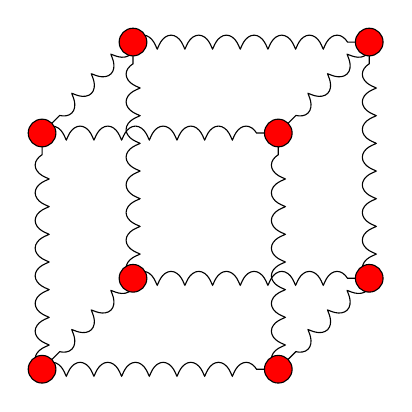
\begin{tikzpicture}

    \draw[-,snake=coil] (0,0 ,0) -- (0,3 ,0);
    \draw[-,snake=coil] (0,0 ,3) -- (0,3 ,3);
	 \draw[-,snake=coil] (3,0 ,0) -- (3,3 ,0);
	 \draw[-,snake=coil] (3,0 ,3) -- (3,3 ,3);
\foreach \y in{0,3}
{
    \draw[-,snake=coil] (0,\y ,0) -- (3,\y ,0);
    \draw[-,snake=coil] (0,\y ,3) -- (3,\y ,3);
	 \draw[-,snake=coil] (0,\y ,0) -- (0,\y ,3);
	 \draw[-,snake=coil] (3,\y ,0) -- (3,\y ,3);

	 \filldraw[fill=red, draw=black] (0, \y, 0) circle (5pt);
	 \filldraw[fill=red, draw=black] (3, \y, 0) circle (5pt);
	 \filldraw[fill=red, draw=black] (0, \y, 3) circle (5pt);
    \filldraw[fill=red, draw=black] (3, \y, 3) circle (5pt);
}

\end{tikzpicture}

\caption{Zbiór punktów masy z przykładowym układem sprężyn.}
\end{figure}

%
% Równanie ogólne siły działającej na punkt masy
%
\begin{equation}
\vec{F}_{i} = \sum_{j} \vec{g}_{ij} + \vec{f}^{d}_i + \vec{f}^{ex}_{i}.
\end{equation}

W powyższym równaniu na punkt masy w danej chwili $t$ działają siły:
\begin{itemize}
\item  Sprężystości $\vec{g}_{ji}$ generowane przez sprężyny zawieszone między sąsiadującymi punktami.

\begin{equation}
\vec{g}_{ij} = k_s (|\vec{x}_{ij}| - l_{ij})\frac{\vec{x}_{ij}}{|\vec{x}_{ij}|},
\end{equation}
gdzie $\vec{x}_{ij} = \vec{x}_i - \vec{x}_j$, jest wektorem różnicy położeń
między sąsiadującymi punktami masy. Siła sprężystości w modelu jest zgodna z
prawem Hook'a, czyli jest proporcjonalna do odchylenia sprężyny od jej
spoczynkowej długości $l_{ij}$. Współczynnik $k_s$ jest współczynnikiem
sprężystości i charakteryzuje materiał z którego składa się symulowane ciało.

\item Siła tłumienia $f^{d}_i$ wynikająca z faktu, iż symulowanie ciało nie jest
doskonale elastyczne i nie zachowuje energii układu. (tzn. energia mechaniczna
		jest transformowana w energię wewnętrzną ciała, co oznacza że z punktu
		widzenia symulacji energia mechaniczna nie jest zachowana.)

\begin{equation}
\vec{f}^{d}_i = k_d(\vec{v}_j - \vec{v}_i),
\end{equation}
gdzie $\vec{v}_i - \vec{v}_j$ jest wektorem prędkości względnej dwóch punktów
masy połączonych sprężynami, a $k_d$ jest współczynnikiem tłumienia charakterystycznym dla symulowanego materiału.

\item Siły zewnętrzne $\vec{f}^{ex}_{i}$ działające na punkt materialny, takie jak np. grawitacja.
\end{itemize}. 

Ewolucja modelu opisana jest równaniem różniczkowym drugiego rzędu:
\begin{equation}
\ddot{\vec{x}} = \frac{\vec{F}}{m}, gdzie \vec{F} = \sum_i \vec{F}_i
\end{equation}
i może być rozwiązany jednym z wielu algorytmów numerycznych.
Jedną z najczęściej wykorzystywanych metod jest algorytm Verleta, który cechuje się prostą
implementacją, dając jednocześnie wystarczająco dokładne rozwiązania. Badania
przeprowadzone w \cite{var} pokazały, że algorytm Verleta okazał się
najwydajniejszy w porównaniu z innymi metodami numerycznymi, dlatego też będzie
stosowany w niniejszej pracy.

Wzór na pozycję punku masy $i$ w czasie $t + dt$ jest w tym algorytmie wyrażona wzorem:

% Wzór na dynamikę punktu w modelu (Verlet)
\begin{equation}
\vec{x}_i(t + dt) = \frac{\vec{F}_i(t)}{m} dt^2 + 2\vec{x}_i(t) - \vec{x}_i(t -
		dt) + O(dt^4)
\end{equation}

W podstawowej metodzie Verleta błąd aproksymacji nowych pozycji punktów masy
jest rzędu $O(dt^4)$. Oznacza to, że przy wyliczaniu nowych pozycji nie jest
uwzględniany wpływ pochodnych 4 rzędu i wyższych z rozwinięcia funcji
$\vec{x}_i(t)$ w szereg Taylora. Wariant podstawowy metody Verleta posiada
 jednak wadę - nie wylicza bezpośrednio prędkości, które mogę być potrzebne do
 wyliczania np. sił działających na ciało. Rozwiązaniem problemu jest inna
 wersja metody Verleta, zwana prędkościową:

% Wzór na dynamikę punktu w modelu (prędkościowy Verlet)
\begin{eqnarray}
\vec{x}_i(t + dt) = \frac{\vec{F}_i(t)}{2m} dt^2 + \vec{x}_i(t) + \vec{v}_i(t)dt
+ O(dt^2)\\
\vec{v}_i(t + dt) = \frac{\vec{F}_i(t + dt) + \vec{F}_i(t)}{2m}dt + \vec{v}_i(t)
+ O(dt^2)
\end{eqnarray}

%
% MODYFIKACJE MODELU
%
\subsection{Modyfikacje modelu}

\subsubsection{Siła tłumienia}
Definicja siły tłumienia jako wielkości proporcjonalnej do różnicy prędkości między dwoma punktami masy w
jest rzadko stosowana, ze względu na wiele niepożądanych
własności. Umożliwia ona np. aby wektor siły tłumienia nie było równoległy do 
wektora różnic położeń dwóch punktów masy połączonych spręzyną.
Efektem tego, jest np. tłumienie obrotu ciała wokół nieruchomego punktu masy, tak jak
przedstawiono na rys. \ref{tlumienie}.

\begin{figure}[ht]
\centering
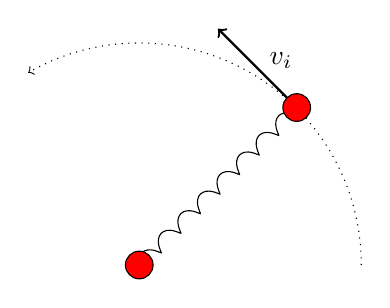
\begin{tikzpicture}

\draw[->,dotted,] (2.82,0) arc (0:120:2.82) ;
\draw[-,snake=coil] (0,0) -- (2,2);
\draw[->, thick] (2,2) -- (1,3);
\filldraw[fill=red, draw=black] (0,0) circle (5pt);
\filldraw[fill=red, draw=black] (2,2) circle (5pt);
\draw (1.8, 2.6) node {$v_i$};
\end{tikzpicture}


\caption{Rotacja wokół nieruchomego punktu}
\label{tlumienie}
\end{figure}

Według \cite{pbdo} przyjęcie prostej różnicy prędkości punktów w przypadku
symulacji materiałów tłumi też ich inne pożądane własności, takie jak podatność na gięcie
i marszczenie. Dlatego też warunek na siłę tłumienia zdefiniujemy jako:
\begin{equation}
\vec{f}^{d}_i = k_d (\frac{\vec{v}_{ij} \cdot
		\vec{x}_{ij}}{\vec{x}_{ij} \cdot \vec{x}_{ij}}) \vec{x}_{ij},
\end{equation}

gdzie $\vec{v}_{ij} = \vec{v}_i - \vec{v}_j$, jest prędkością względną, a $\vec{v}_{ij} \cdot \vec{x}_{ij}$ jest 
składową prędkością względnej w kierunku $\vec{x}_{ij}$. Definicja nakłada zatem
ograniczenie, iż siła tłumienia może działać tylko w kierunku wyznaczonym przez
sprężynę.

\subsubsection{Zachowanie objętości}
Kolejnym, istotnym aspektem symulacji ciała miękkiego jest zachowanie jego
objętości. System punktów mas i sprężyn nie symuluje obiektów posiadających
objętość, także często może się zdarzyć, że układ znajdzie się w stanie
stabilnym, jednak różnym od wyjściowego. W praktyce często oznacza to, że w
wyniku działania dużych sił elementy modelu zostaną obrócone lub zapadną się.
Przykład tego jest przedstawiony na rysunku \ref{stany}.

\begin{figure}[ht]
\centering
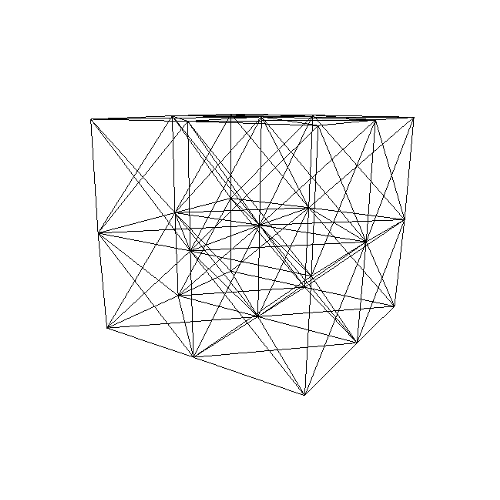
\includegraphics[width=7cm, height=7cm]{images/stabilny.png}
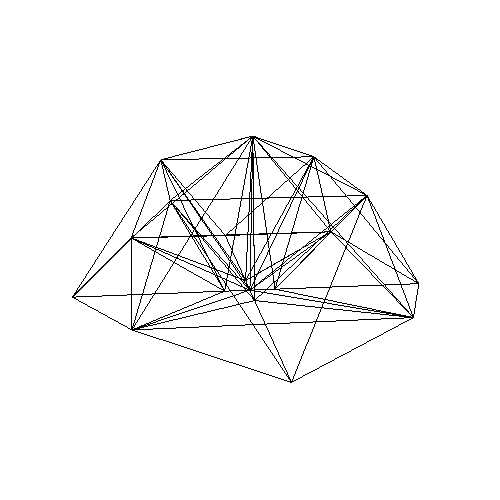
\includegraphics[width=7cm, height=7cm]{images/niestabilny.png}
\caption{Dwa stany stabilne dla sześciennego modelu.}
\label{stany}
\end{figure}

Rozwiązaniem problemu przechodzenia układu między stanami stabilnymi okazało się
wprowadzenie sztucznej siły, pozwalającej zachować objętość. Takie podejście po
raz pierwszy zaproponowano w \cite{rmofa}. Autorzy publikacji pogrupowali
znajdujące się w układzie punkty masy w obiekty dla których można było
zdefiniować objętość. Następnie w zależności od różnicy pomiędzy objętością
spoczynkową a aktualną generowana była siła oddziałująca na punkty masy. Kierunek
tej siły jest zgodny z działaniem pewnej z góry zdefiniowanej normalnej. W
\cite{isodb} autorzy przedstawiają bardziej ogólny przypadek przyjmując, że
obiektem posiadającym objętość jest czworościan.Wierzchołki figury są punktami
masy, a krawędzie sprężynami. Siła zachowawcza działająca na dany punktu masy
$i$ czworościanu, określa się wzorem:

\begin{equation}
\vec{F}_i^d = d_v ( v - v_0) \vec{n}_i,
\end{equation}
gdzie $v$ jest aktualną objętością symulowanego czworościanu, $v_0$ jest jego
spoczynkową objętością a $d_v$ jest arbitralnie zdefiniowaną stałą. $|vec{n}_i$ jest
to normalna przeciwległej ściany czworościanu. Podana metoda pozwala uniknąć
odwrócenia wierzchołków symulowanego obiektu, ponieważ w takim przypadku
obliczona objętość będzie ujemna i powstałaby duża siła $F_i^d$, która wymusi powrót
układu do stanu oryginalnego\cite{isodb}.

\subsection{Zależność od topologii}
W analizowanym modelu topologia połączeń punktów mas sprężynami jest z góry
zdefiniowana. Można powiedzieć, że jest to kolejny parametrem symulacji, który w
istotny sposób decyduje o jej jakości. Modelując wewnętrzną strukturę ciała możemy określić jego fizyczną
charakterystykę. Na przykład, symulując elastyczny sześcian i dodając dodatkowe
połączenia między punktami masy w jednej płaszczyźnie otrzymamy obiekt różnie
podatny na odkształcanie w zależności od kierunku działania siły. Taką
mechaniczną właściwość ciała nazywany anizotropią. Anizotropia stanowi bardzo
ciekawy przykład własności mechanicznej materiału, której implementacja w modelu
punktów mas i sprężyn jest często problematyczna. 

Idealny model powinien umożliwiać symulowanie materiałów izotropowych (o
		własnościach mechanicznych niezależnych od kierunki działań siły) jak i
anizotropowych. Poprzez możliwość manipulacji rozmieszczeniem punktów
materialnych, sposobami połączeń sprężynami czy manipulowaniem stałymi
sprężystości, model dostarcza narzędzi do implementacji tych własności. Nie
mniej jednak niektóre własności mogą pojawiać się wbrew wcześniejszym
założeniom. Przykład niepożądanej anizotropii, otrzymanej poprzez różne
struktury wewnętrzne modelu przedstawiono na rys. \ref{anizotropia}.

\begin{figure}[ht]
\centering
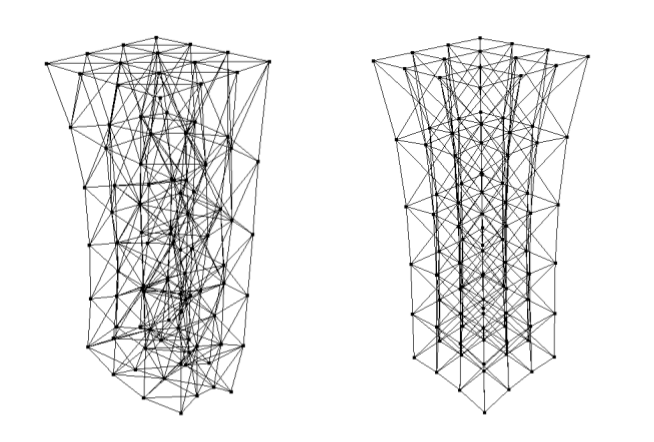
\includegraphics[scale=0.5]{images/anisotropy.png}
\caption{Różnice własności anizotropijne dwóch prostopadłościanów
	przytwierdzonych górną podstawą i poddanych sile grawitacji. Lewo:
		Czworościenna siatka połączeń. Prawo: Sześciościenna siatka połączeń. Źródło: \cite{ca}}
\label{anizotropia}
\end{figure}

Okazuje się, że kalibracja parametrów modelu nie jest trywialna. W \cite{usa}
autorzy proponują metodę kalibracji poszczególnych stałych sprężystości sprężyn.
Ich metoda pozwala na symulację zarówno układów izotropowych jak i anizotropowych,
jednak, jak sami autorzy wskazują jest złożona obliczeniowo, a w publikacji
został zaprezentowany tylko przykład dla siatek dwuwymiarowych. Inne podejście
w swojej publikacji przedstawili francuscy badacze wykorzystując do estymacji
parametrów sprężystości algorytmy genetyczne.\cite{ei}

Alternatywne podejście, odchodzące nieco od klasycznego modelu punktów mas i
sprężyn, zostało przedstawione w publikacji D. Bourguignon i M-P. Cani
\cite{ca}. Metoda ta, pochodna systemu punktów mas i sprężyn, pozwala na
definiowanie własności mechanicznych symulowanych obiektów niezależnie od
przyjętej geometrii czy topologii. Pozwala to na użycie do symulacji obiektów
utworzonych w programach do modelowania 3D i co ważniejsze, odciążenia grafika z
konieczności uwzględnienia podczas pracy fizycznych charakterystyk
modelu.\cite{ca}

Metoda ta zakłada, że wszystkie punkty masy w modelu są pogrupowane w tzw. jednostki
objętości (volume element), którymi najczęściej są czworościany. Dla każdej
jednostki wyznacza się tymczasowe punkty masy położone wzdłuż stałych,
		  predefiniowanych osi. Umiejscowienie osi ma odzwierciedlać mechaniczną
		  charakterystykę obiektu. Z reguły stosuje się standardowo 3 osie,
		  jednak możliwa jest też ich większa ilość \cite{ca}. Sposób
		  wyznaczania punktów przecięcia przedstawiony jest na rysunku
		  \ref{anizotropia-czworoscian}.

\begin{figure}[ht]
\centering
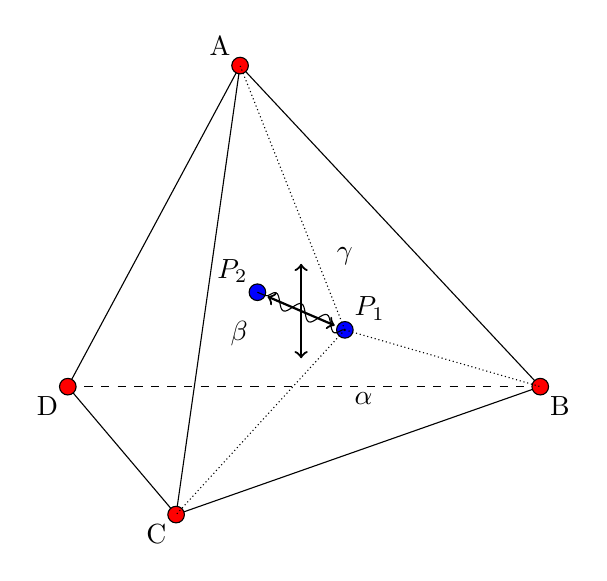
\begin{tikzpicture}

\coordinate (A) at (0, 0, 0);
\coordinate (B) at (6, 0, 0);
\coordinate (C) at (3, 0, 4.22);
\coordinate (D) at (3, 4.89, 2.11);

\draw[-] (D) -- (B) -- (C) -- (D) -- (A) -- (C);
\draw[-, dashed] (A) -- (B);

\filldraw[fill=red, draw=black] (A) circle (3pt);
\filldraw[fill=red, draw=black] (B) circle (3pt);
\filldraw[fill=red, draw=black] (C) circle (3pt);
\filldraw[fill=red, draw=black] (D) circle (3pt);

\node[above left] at (D) {A};
\node[below right] at (B) {B};
\node[below left] at (C) {C};
\node[below left] at (A) {D};

%intersection points
\coordinate (I1) at (barycentric cs:D=0.5,B=0.7,C=0.5);
\coordinate (I2) at (barycentric cs:A=0.7,B=0.5,D=0.5);
\coordinate (Imid) at (barycentric cs:I1=0.5,I2=0.5);

\filldraw[fill=blue, draw=black] (I1) circle (3pt);
\filldraw[fill=blue, draw=black] (I2) circle (3pt);
\node[above right] at (I1) {$P_1$};
\node[above left] at (I2) {$P_2$};
\node[below=25pt, right] at (I1) {$\alpha$};
\node[below=15pt, left] at (I2) {$\beta$};
\node[right, above=20pt] at (I1) {$\gamma$};

\draw[-,snake=snake] (I1) -- (I2);
\draw[<->,thick, shorten >=4pt, shorten <=4pt] (I1) -- (I2);
\draw[->,thick] (Imid) -- ++(0,0.6,0);
\draw[->,thick] (Imid) -- ++(0,-0.6,0);

\draw[-,densely dotted] (I1) -- (C);
\draw[-,densely dotted] (I1) -- (D);
\draw[-,densely dotted] (I1) -- (B);


\end{tikzpicture}

\caption{Wyznaczanie punktu przecięcia z osiami w czworościanie.}
\label{anizotropia-czworoscian}
\end{figure}

Przedstawiony czworościan posiada zdefiniowane dwie osie. Wyznaczono też dwa
punkty przecięcia $P_1$ oraz $P_2$ z osią poziomą figury. W celu zapamiętania
pozycji punktów przecięcia wyznacza się współczynniki kombinacji liniowej z
wierzchołkami tworzącymi ścianę. $P_1 = \alpha * A + \beta *B + \gamma *C$.
Współczynniki te muszą być wyznaczane dla czworościanu znajdującego się w stanie
spoczynku. Punkty przecięcia traktowane są odtąd jak nowe punkty masy. Działają
na nie siły wewnętrzne i zewnętrzne układu. Dwa punkty (zaznaczonymi na rys.
		\ref{anizotropia-czworoscian} kolorem niebieskim) zostają w istocie
połączone sprężyną.

Następnie dokonuje się omawianych w poprzednich podrozdziałach obliczeń sił
działających na punkt przecięcia. Mając dane współczynniki kombinacji liniowej,
	wyznaczyć można siły działające na punkty masy $A,B,C, D$ pierwotnie zdefiniowane w modelu. 

\begin{figure}[ht]
\centering
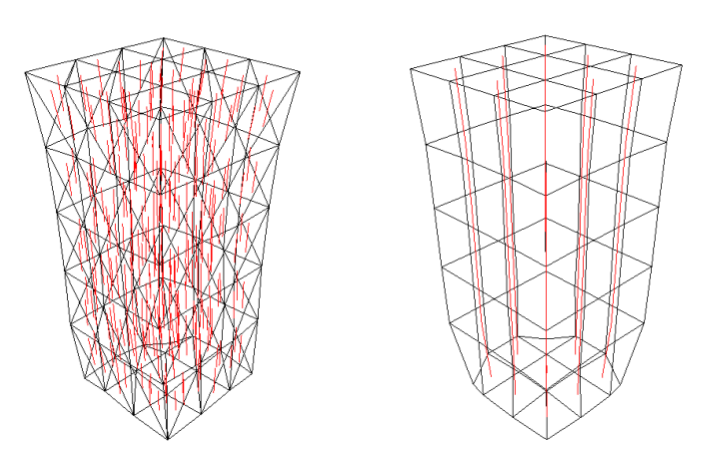
\includegraphics[scale=0.5]{images/fixed_anisotropy.png}
\caption{Porównanie dwóch zastosowanych siatek w obiekcie przytwierdzonym górną podstawą i poddanemu sile grawitacji. W modelu wykorzystano metodę D. Bourguignon i M-P. Cani, Źródło: \cite{ca}}
\label{anizotropia-czworoscian-fix}
\end{figure}


\chapter{Wybrana metoda symulacji ciała miękkiego}

\section{Kryteria wyboru modelu}

Wybór metody symulacji uzależniony jest od zakresu zjawisk fizycznych które mają
być jej przedmiotem. Zanim przedstawiona zostanie wybrana metoda wymienione będą
kryteria którymi kierowałem się przy jej wyborze.  Pragnę też zaznaczyć, że
wybór ten nastąpił w głównej mierze metodami prób i błędów.  Większość z
poznanych przeze mnie metod została zaimplementowana i w przypadku niemożności
uzyskania pożądanych efektów wizualnych lub wydajnościowych wyszukiwana była
inna.

Pierwszym kryterium jakim kierowałem się przy wyborze metody było zawężenia
przedmiotu symulacji do ciał posiadających objętość. Wiele z metod symulacji
ciała miękkiego ukierunkowana jest na symulację ciał nie posiadających objętości
- takich jak włosy czy materiały. Metody te zaaplikowane do obiektów
posiadających objętość często nie dawały oczekiwanych rezultatów (miało to
		np. miejsce w przypadku omawianej później dynamiki pozycyjnej w formie
		zaproponowanej przez jej autorów). Dodatkowo większość z posiadanych przez nie
własności trzeba było wyeliminować ze względu na charakter symulowanego zjawiska
- przykładem jest np. efekt marszczenia powierzchni.

Kolejnym kryterium, a właściwie uproszczeniem było założenie, że symulowany
obiekt będzie jednorodny pod względem wypełnienia, czy inaczej, materiału z
którego jest zbudowany. Pozwala to na uniknięcia modelowania, często
nietrywialnego, właściwości fizycznych modelu, co z pewnością wykroczyłoby poza
temat tej pracy. 

% złożone obiekty o skomplikowanej siatce
Innym istotnym wymaganiem jest umożliwienie symulowania obiektów
przygotowanych w programach do modelowania 3D. Obiekty takie często składają się
wielu tysięcy wierzchołków, które posiadają własne współrzędne teksturowania,
czy normalne. Implikacją tego założenia jest fakt, że poszukiwana metoda musi być
metodą Lagrange'a symulującą dynamikę wierzchołków trójwymiarowego modelu.
Dodatkowe informacje związane z modelem, takie jak połączenia między
wierzchołkami czy wierzchołki tworzące trójkąty mogą być wykorzystane w
symulacji.

% zakres degeneracji
Kolejnym wymaganiem jest przyjęcie, że symulowane ciało miękkie poddane
działaniu sił będzie odkształcane tylko w średnim zakresie. W
przypadku gdy siły zewnętrzne przestają działać na ciało, siły wewnętrzne
powinny sprowadzić obiekt do formy nieodkształconej. Takie założenie upraszcza
symulację gdyż wyklucza trwałą degenerację siatki obiektu.

% przeznaczona do symulacji czasu rzeczywistego stabilna do zastosowań
Najważniejszym wymaganiem jakie brane było pod uwagę przy wyborze metody jest możliwość
zastosowania jej do symulacji czasu rzeczywistego. Metody złożone obliczeniowo takie
jak przytaczane w rozdziale 2 Metody Continuum nie spełniają tego kryterium.
Również metody wymagające zaawansowanej obróbki modelu - taka jak np. System
Sprężyn wymagają zdefiniowania wewnętrznej struktury obiektu, co wiąże się z
generowaniem znacznej ilości cząstek poddanych symulacji. 

Z moich eksperymentów z wypełnianiem modelu sześcienną siatką i użyciem Systemu Sprężyn wynika, że
gęste wypełnienie średniej złożoności modelu punktami wewnętrznymi powoduje
zbytnie usztywnienie obiektu i znacząco spowalnia symulację. W przeciwieństwie,
gdy wnętrze modelu jest rzadko wypełnione cząstkami wewnętrznymi wyjściowa
siatka modelu podlega znacznej degeneracji. Znalezienie optymalnej gęstości
siatki oraz współczynników sprężystości sprężyn odbywało się drogą eksperymentów.

% skalowana do gpu
Tematem tej pracy jest również poznanie i zastosowanie technologii CUDA. Dlatego też
ostatnim kryterium jakie brane było pod uwagę przy wyborze metody symulacji jest
możliwość wykorzystania GPU do obliczeń.

% skad wzialem metode czyja to, kiedy skad
Jako źródło informacji o dostępnych metodach wykorzystywany był głównie
internet. Jak to zostało wcześniej napisane, nie są znane mi żadne książki
poruszające tematykę symulacji ciał miękkich w grafice komputerowej. Mimo
niedostępności poszukiwanego kompendium wiedzy dostępne są trzy bardzo dobre
artykuły stanowiące przekrój przez szereg opublikowanych metod: \cite{TR97-19},
	\cite{pbdo}, \cite{survey}. Cennym źródłem informacji są też materiały
	publikowane konferencyjne publikowane na stronie \textit{www.siggraph.org}.

% klasyfikacja tej metody - Lagrange geometryczno fizyczny
Zaimplementowana w tej pracy metoda bazuje na artykule \textit{Robust
	Real-Time Deformation of Incompressible Surface Meshes}\cite{diziol},
opublikowanym na konferencji SIGGRAPH w 2011r. Wybrana metoda jest wg
klasyfikacji z rozdziału 2 metodą Lagrange'a posiadająca zarówno elementy
fizyczne jak i niefizyczne. Elementami fizycznymi jest pojawianie się sił w
momencie gdy obiekt zmienia swoją objętość oraz siły grawitacji. Za część
niefizyczną, uznany jest tzw. \textit{Shape Matching}, czyli metoda geometryczna
oddziałująca na cząstki modelu w taki sposób aby zminimalizować ich odchylenie
ich położeń od stanu wejściowego oraz technika zachowania objętości. Obie
techniki będą dokładniej omawiane w rozdziałach \ref{sec:shape} i \ref{sec:vol}

% dlaczego powinna byc szybka nie potrzeba wypelniac obiektu puntkami - operuje bezposrednio na powierzchni siatki
Ważniejszą jednak zaletą wybranego modelu jest fakt, że w przeciwieństwie do
Systemu Sprężyn symulowane obiekty nie muszą mieć
zdefiniowanej struktury wewnętrznej. Pozwala to znacząco przyspieszyć symulację
unikając generowania i symulacji znacznej ilość cząstek, które odpowiadają tylko za
utrzymanie fizycznych właściwości obiektu. Metoda ta operuje bezpośrednio na
trójkątnej siatce, co pozawala wczytać obiekt bezpośrednio z formatu modeli
3D.

% dlaczego powinna byc stabilna - brak sil, dynamika z constraintami
Kolejną zaletą użytej techniki symulacji jest jej stabilność, która wynika z
nowatorskiego podejścia do rozwiązywania równań ruchu. Nie posiada ona
wielu źródeł niestabilności typowych dla modelu Systemu Sprężyn.
Dokładne omówienie symulowania dynamiki wybranej metody nastąpi w rozdziale
\ref{sec:dyn}.

% dlaczego jest dobra na gpu
Ostatnią zaletą jest też możliwość efektywnej implementacji wybranej metody na
procesorach graficznych. Dobra lokalność przetwarzanych danych sprawia, że
możliwe jest pełne wykorzystanie procesora graficznego, co w połączeniu z
techniką redukcji złożoności algorytmu zaproponowaną przez autorów, czyni ją
idealną do zastosowania w symulacjach czasu rzeczywistego.

\section{Zachowanie kształtu}
\label{sec:shape}
Dopasowanie kształtu (ang. Shape Matching) jest geometryczną techniką
zaproponowaną po raz pierwszy w 2005 r. przez Muller'a \cite{shape}. Służy ona do
symulowania sił wewnętrznych ciała poddanego deformacji. Metoda ta zamiast
generować siły działające na cząstki, tak jak to ma miejsce w przypadku
sprężyn w modelu Systemu Sprężyn, definiuje docelowe pozycje cząstek - $g_i$.
Pozycje te powstają w wyniku próby dopasowania konfiguracji 
pozycji cząstek ciała w stanie niezdeformowanym do aktualnej.

Wyliczone docelowe pozycje $\vec{g}_i$ wykorzystywane są w symulacji do "przyciągania"
aktualnych pozycji cząstek. W przypadku gdy docelowe pozycje cząstek stają się
natychmiastowo aktualnymi uzyskamy efekt dynamiki ciała sztywnego.

\begin{figure}[ht]
\centering
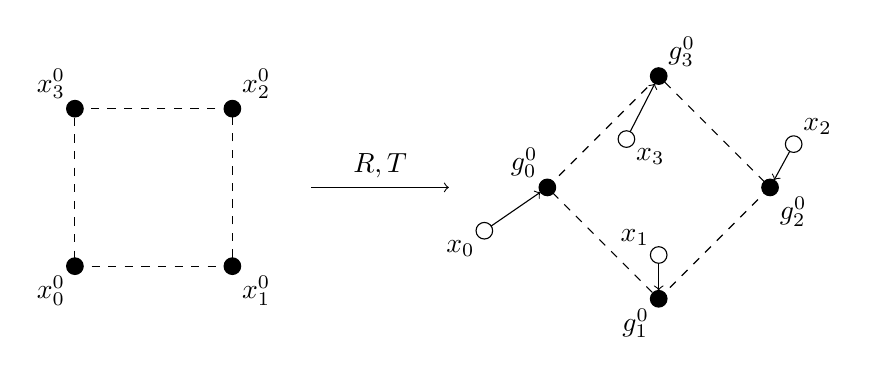
\begin{tikzpicture}

	\coordinate (A) at (0, 0, 0);
	\coordinate (B) at (2, 0, 0);
	\coordinate (C) at (2, 2, 0);
	\coordinate (D) at (0, 2, 0);

	\draw[-,dashed] (A) -- (B) -- (C) -- (D) -- (A);

	\filldraw[fill=black, draw=black] (A) circle (3pt);
	\filldraw[fill=black, draw=black] (B) circle (3pt);
	\filldraw[fill=black, draw=black] (C) circle (3pt);
	\filldraw[fill=black, draw=black] (D) circle (3pt);

	\node[above left] at (D) {$x^0_3$};
	\node[below right] at (B) {$x^0_1$};
	\node[above right] at (C) {$x^0_2$};
	\node[below left] at (A) {$x^0_0$};

	% arrow
	\coordinate (R1) at (3, 1, 0);
	\coordinate (R2) at (4.75, 1, 0);
    \draw[->] (R1) -- (R2) node[midway,above] {$R, T$};

	% transformed

	\coordinate (A1) at (6, 1, 0);
	\coordinate (B1) at (7.4142, 2.4142, 0);
	\coordinate (C1) at (8.8284, 1, 0);
	\coordinate (D1) at (7.4142, -0.4142, 0);

	\draw[-,dashed] (A1) -- (B1) -- (C1) -- (D1) -- (A1);

	\filldraw[fill=black, draw=black] (A1) circle (3pt);
	\filldraw[fill=black, draw=black] (B1) circle (3pt);
	\filldraw[fill=black, draw=black] (C1) circle (3pt);
	\filldraw[fill=black, draw=black] (D1) circle (3pt);

	\node[below left] at (D1) {$g^0_1$};
	\node[above right] at (B1) {$g^0_3$};
	\node[below right] at (C1) {$g^0_2$};
	\node[above left] at (A1) {$g^0_0$};

	\coordinate (X1) at (5.2, 0.45, 0);
	\coordinate (X2) at (7.0042, 1.6142, 0);
	\coordinate (X3) at (9.1284, 1.55, 0);
	\coordinate (X4) at (7.4142, 0.142, 0);

	\filldraw[fill=white, draw=black] (X1) circle (3pt);
	\filldraw[fill=white, draw=black] (X2) circle (3pt);
	\filldraw[fill=white, draw=black] (X3) circle (3pt);
	\filldraw[fill=white, draw=black] (X4) circle (3pt);

	\node[below left] at (X1) {$x_0$};
	\node[below right] at (X2) {$x_3$};
	\node[above right] at (X3) {$x_2$};
	\node[above left] at (X4) {$x_1$};

    \draw[shorten >=3pt,shorten <=3pt,->] (X1) -- (A1);
    \draw[shorten >=3pt,shorten <=3pt,->] (X2) -- (B1);
    \draw[shorten >=3pt,shorten <=3pt,->] (X3) -- (C1);
    \draw[shorten >=3pt,shorten <=3pt,->] (X4) -- (D1);

\end{tikzpicture}

\caption{Geometryczne dopasowanie kształtu do zdeformowanych punktów w Shape Matching.}
\label{shape-matching}
\end{figure}

Ideę shape matching przedstawia rysunek \ref{shape-matching}. Punkty w stanie
niezdeformowanym $\vec{x}^0_i$ są dopasowywane do zdeformowanych pozycji
$\vec{x}_i$ za
pomocą macierzy rotacji i wektorów translacji. 
Formalnie koncepcję Shape Matchingu autorzy w \cite{shape} zdefiniowali jako problem minimalizacji
funkcji:
\begin{equation}
E^2 = \sum_{i} m_i ||R (x^0_i - t^0) - (x_i - t) ||^2,
\label{min}
\end{equation}

gdzie $t^0$ i $t_i$ są wektorami translacji, a $R$ jest macierzą
rotacji.

Przedstawiony problem sprowadza się do minimalizacji błędu średniokwadratowego.
Wyrażenie z (\ref{min}) można przedstawić jako funkcję trzech zmiennych:
\begin{equation*}
\phi(R, t, t^0) = \sum_{i} m_i ||R (x^0_i - t^0) - (x_i - t) ||^2,
\end{equation*}

Okazuje się, że znalezienie wartości wektorów $t$ i $t^0$ w
wyrażeniu (\ref{min}) jest możliwe. Muller \cite{shape} podaje, że optymalnymi
wektorami translacji $t^0$ i $t$ są odpowiednio środek masy obiektu
niezdeformowanego (konfiguracja spoczynkowa) i środek masy
ciała w aktualnej konfiguracji. Pokazanie tego rozwiązania polega na
wyliczeniu gradientów funkcji $\phi$ po zmiennych $t$ i $t^0$ i przyrównaniu ich
do zera.

Zanim zostanie przedstawiony dowód że, położenia środków mas są optymalnymi wektorami
translacji, przypomniane zostaną wzory na pochodne cząstkowe wraz z ich
wektorowymi odpowiednikami. Zakładając że dane mamy funkcje $f: R^n \to R^m$,
$g: R^n \to R^m$ i $h = f^T g$, gdzie $h: R^n \to R^1$. Gradient
funkcji $h$ wyraża się wzorem:
\begin{equation*}
\partial h = f^T \partial g + g^T \partial f
\end{equation*}
gdzie $\partial f$ to macierz Jacobiego (pochodnych cząstkowych), a $f^T$ jest
oznaczeniem transpozycji funkcji.

W przypadku gdy funkcje $f = g$, gradient ma postać:
\begin{equation}
\partial h = 2 f^T \partial f,
\label{part}
\end{equation}

Wprowadzając nowe oznaczenia:
$$ v = R (x^0_i - t^0) - (x_i - t)$$
$$ \phi = \sum_i m_i v^T v$$ 
i uwzględniając własność (\ref{part}), gradient funkcji $\phi$ po
zmiennych $t^0$ i $t$ zapiszemy:
\begin{eqnarray*}
\nabla_{t^0} \phi = 2 \sum_i m_i (R (x^0_i - t^0) + t - x_i)^T (-R)\\
\nabla_{t} \phi = 2 \sum_i m_i (R (x^0_i - t^0) + t - x_i)^T\\
\end{eqnarray*}

Transponując obie strony otrzymujemy:
\begin{eqnarray*}
\nabla_{t^0}^T \phi = -2 \sum_i m_i R^T (R (x^0_i - t^0) + t - x_i)\\
\nabla_{t}^T \phi = 2 \sum_i m_i (R (x^0_i - t^0) + t - x_i)\\
\end{eqnarray*}

W celu wyliczenia wartości $t$ i $t^0$ przyrównujemy gradient do zera:
\begin{eqnarray}
\label{d1}
\nabla \phi_{t^0} = 0 \Leftrightarrow \sum_i m_i R^T (R (x^0_i - t^0) + t - x_i) = 0\\
\label{d2}
\nabla \phi_{t} = 0 \Leftrightarrow \sum_i m_i R (x^0_i - t^0) + t - x_i = 0
\end{eqnarray}

Można łatwo zauważyć że równania (\ref{d1}) oraz (\ref{d2}) są od siebie liniowo
zależne. Przekształcając równanie (\ref{d2}) otrzymujemy:

\begin{eqnarray*}
\sum_i m_i (R (x^0_i - t^0) + t - x_i) = 0\\
\sum_i m_i R x^0_i - \sum_i m_i R t^0 + \sum_i m_i t - \sum_i m_i x_i = 0\\
R \sum_i m_i t^0 - \sum_i m_i t = R \sum_i m_i x^0_i - \sum_i m_i x_i\\
\end{eqnarray*}
Ostatecznie równanie spełniające warunek optymalizacji (\ref{min}) dla wektorów $t$
i $t^0$ możemy zapisać jako:
\begin{equation}
\label{tt0}
R t^0 - t = R \frac{\sum_i m_i x^0_i}{\sum_i m_i} - \frac{\sum_i m_i
	x_i}{\sum_i m_i}
\end{equation}

Z równania (\ref{tt0}) wynikają następujące wnioski. Nie istnieje unikalna para
wektorów
$t$ i $t^0$ spełniająca warunek minimalizacji wyrażenia (\ref{min}). Rozwiązaniem
trywialnym (\ref{tt0}) jest $t = \frac{\sum_i m_i x_i}{\sum_i m_i}$
i $t^0 = \frac{\sum_i m_i x^0_i}{\sum_i m_i}$,
	co dowodzi tezy postawionej w \cite{shape}. Przyjęcie środków mas jako
	wektorów translacji sprawia, że wartości $t$ i $t^0$ minimalizujące
	(\ref{min}) są niezależne od wartości macierzy rotacji $R$.

Ostatnim elementem niezbędnym do wyliczenia docelowych pozycji $g_i$ jest
macierz obrotu $R$. W tym celu musimy wprowadzić następujące oznaczenia:
\begin{eqnarray*}
x_{cm}^0 = \frac{1}{M} \sum_i m_i x_i^0,\\
x_{cm} = \frac{1}{M} \sum_i m_i x_i,\\
M = \sum_i m_i,\\
\vec{q}_i = x_i^0 - x_{cm}^0,\\
\vec{p}_i = x_i - x_{cm}.
\end{eqnarray*}
Używając powyższych oznaczeń i uwzględniając fakt, że wybrane wektory translacji
są niezależne od R wyrażenie (\ref{min}) może być zapisane następująco:
\begin{equation*}
\phi(R) = \sum_i m_i || R\vec{q}_i - \vec{p}_i||^2
\end{equation*}

Wyznaczenie macierzy R odbywa się analogicznie jak w przypadku wektorów
translacji, z jedyną różnicą, że gradient wyznaczony jest teraz po macierzy.
Muller \cite{shape} przy wyliczaniu macierzy $R$, uchyla założenie, że macierz ta
jest tylko macierzą rotacji, a przyjmuje, że jest to macierz transformacji
liniowej. W celu odróżnienia tych dwóch różnych problemów zdefiniujmy problem
ponownie jako:
\begin{eqnarray}
\phi(A) = \sum_i m_i || A \vec{q}_i - \vec{p}_i||^2
\end{eqnarray}

Rozwiązaniem minimalizującym funkcję $\phi$ jest macierz:\cite{shape}
\begin{equation}
A = (\sum_i m_i \vec{p}_i \vec{q}^T_i)(\sum_i m_i \vec{q}_i \vec{q}^T_i)^{-1}
= A_{pq} A_{qq}^{-1}
\end{equation}

Ostatnim krokiem niezbędnym do estymacji punktów docelowych $g_i$ jest
dekompozycja macierzy $A$ i uzyskanie jej składowej rotacji. Jest to możliwe dzięki
użyciu metod takich jak Rozkład Biegunowy (Polar Decomposition) czy Rozkład
według wartości osobliwych (Singular Value Decomposition). Warto też nadmienić,
	że macierz $A_{qq}$ jest macierzą symetryczną i zawiera w sobie tylko
	informacje o skalowaniu, a cała informacja o rotacji jest obecna w
	macierzy $A_{pq}$

Zakładając że macierz $A_{pq}$ jest macierzą odwracalną, używając Rozkładu
Biegunowego możemy macierz zapisać jako:
\begin{equation}
A_{pq} = RS
\end{equation}
gdzie $R$ jest macierzą rotacji, a $S$ macierzą skalowania daną wzorami:
\begin{eqnarray*}
S = \sqrt[2]{A^T_{pq} A_{pq}}\\
R = A_{pq} S^{-1}
\end{eqnarray*}

%Formalnie pozycję $g_i$ wyraża się wzorem:
Ostatecznie pozycje docelowe $g_i$ można obliczyć jako:
\begin{equation}
g_i = R(x_i^0 - x^0_{cm}) + x_{cm}
\end{equation}

\subsection{Modyfikacje}
\label{ssec:region}
Shape Matching w swojej podstawowej formie dokonuje optymalizacji dopasowania
globalnie dla wszystkich punktów symulowanego ciała. Powoduje to jego zbytnie
usztywnienie i dopuszcza tylko wąski zakres deformacji.

Aby rozwiązać powyższe problemy Diziol w swoim artykule \cite{diziol} użył
lokalnego shape-matching. Autor unika globalnego dopasowania poprzez
predefiniowanie małych zbiorów sąsiadujących punktów w ramach których będzie
stosowany shape-matching.  W przypadku gdy cząstka należy do wielu regionów,
		  jako ostateczna docelowa pozycja $g_i$ używana jest średnia z
		  dopasowania z poszczególnych regionów.
\begin{equation}
g_i = \frac{1}{K_i} \sum_j^{K_i} R_j (x^0_i - x^0_{cm_j}) + x_{cm_j}
\end{equation}

\section{Zachowanie objętości}
\label{sec:vol}
Symulacja ciała miękkiego bez obostrzeń na zmiany objętości może
prowadzić do dużych jej zmian i niepożądanych wizualnie efektów. 
Aby temu zapobiec do modelu wprowadzona będzie siła wewnętrzna pojawiająca się w
przypadku gdy objętość ciała jest różna od objętości spoczynkowej oznaczonej
przez $V_0$.

Powierzchnię ciała o zamkniętej trójkątnej siatce określonej na jego powierzchni definiuje
się jako: \cite{diziol}
\begin{equation}
\label{obj}
\frac{1}{3} \sum_i^m A_i (a_i + b_i + c_i)^T n_i = 3V
\end{equation}
gdzie $m$ jest ilością trójkątów stanowiących siatkę, a punkty $a_i$, $b_i$,
	  $c_i$ wierzchołkami i-tego trójkąta, $A$ jego powierzchnią, a $n_i$
	  normalną trójkąta.

W pracy \cite{diziol} zdefiniowana jest funkcja ograniczenia nałożona na
objętość ciała postaci:
\begin{equation}
\label{cons}
C(X) = \frac{1}{3} \sum_i^m A_i (a_i + b_i + c_i)^T n_i - 3V_0 = 0
\end{equation}
gdzie $V_0$ jest objętością niezdeformowanego ciała, a $X$ jest zbiorem punktów
siatki. W przypadku gdy pewna konfiguracja punktów $\tilde{X} = [x_1, x_2,...,
	x_n] $ ciała generuje
objętość różną od $V_0$, wtedy należy znaleźć takie przesunięcie punktów $\Delta
\tilde{X}$, tak by spełniona była równość 
$$C(\tilde{X} + \Delta \tilde{X}) = 0$$

Funkcja ograniczenia (\ref{cons}) może zostać aproksymowana przez:
\begin{equation}
\label{e1}
C(X + \Delta X) \approx C(X) + \nabla_X C(X) \Delta X
\end{equation}

Zakładając, że przesunięcie $\Delta X$ może występować tylko wzdłuż gradientu $\nabla_X
C(X)$ otrzymujemy dodatkową równość:
\begin{equation}
\label{e2}
\Delta X = \lambda \nabla_X C(X)
\end{equation}

Rozwiązując układ równań (\ref{e1}) i (\ref{e2}) otrzymujemy ostateczną formułę
opisujące przemieszczenie $\Delta X$ rozwiązujące więzy na objętość:
\begin{equation*}
\Delta X = - \frac{C(X)}{||\nabla_p C(X)||^2} \nabla_X C(X)
\end{equation*}

Indywidualne przemieszczenie $x_i$ mogą zostać wyliczone z formuły:
\begin{equation}
\Delta x_i = - \frac{C(X)}{\sum_j ||\nabla_{x_j} C(X)||^2} \nabla_{x_i} C(X)
\end{equation}

Aby ustalić wartość gradientu przekształcimy wyrażenie (\ref{obj}) w taki sposób,
	aby zamiast sumowania po trójkątach sumowała po punktach siatki:
\begin{equation}
\label{dd}
\frac{1}{3} \sum_i^m A_i (a_i + b_i + c_i)^T n_i = \frac{1}{3} \sum_i^n x_i^T
\tilde{n}_i
\end{equation}
gdzie $\tilde{n}_i = \sum_j A_j n_j$.

Diziol \cite{diziol} nie używa dokładnej formuły na gradient wyznaczony z
(\ref{dd}). Zamiast tego proponuje następujące uproszczenie:
\begin{equation}
\nabla C(X) \approx \frac{1}{3} [\tilde{n}^T_1, \tilde{n}^T_2, ...,
	\tilde{n}^T_n]^T
\end{equation}
Według \cite{diziol} przybliżony gradient nie zmienia znacząco jego wartości, a
pozwala na łatwiejsze jego wyliczenia na GPU.

Ostateczną formułą na przesunięcie związane ze zmianą objętości możemy zapisać:
\begin{equation}
\delta x_i = \frac{\Delta V}{N} \tilde{n}_i
\end{equation}

%$$\iiint\limits_V \nabla \dot f(x) dx = \iint\limits_{\partial V} f(x)^T n(x) dx,$$

%$$\iiint\limits_V \nabla \dot x dx = \iint\limits_{\partial V} x^T n(x) dx = 3 V,$$

%$$ \iint\limits_{\partial V} x^T n(x) dx = \frac{1}{3} \sum_i^m A_i (a_i + b_i +
%		c_i)^T n_i,$$
%$$ \frac{1}{3} \sum_i^m A_i (a_i + b_i + c_i)^T n_i = \frac{1}{3}\sum_i^n x_i^T
%\tilde{n}_i,$$
\section{Dynamika bazująca na pozycji}
\label{sec:dyn}

Zastosowanie geometrycznych technik takich jak wymieniony w rozdziale
\ref{sec:shape} Shape-Matching czy metod zachowujących objętość w \ref{sec:vol}
jest problematyczne z tego względu, że siły działające na ciało nie wynikają
z nich bezpośrednio. Niemożliwe zatem jest jawne zdefiniowanie dynamiki układu
opisanego równaniem różniczkowym postaci $\ddot{\vec{x}} = \vec{F}/m$.

Rozwiązaniem tego problemu może być emulowanie sił poprzez zaczepienie
'wirtualnych' sprężyn pomiędzy punktami docelowymi $g_i$ wynikającymi z ograniczeń
geometrycznych a aktualną pozycją $x_i$ cząstki. Otrzymane w ten sposób
siły działające na ciało mogą być użyte do rozwiązania równań ruchu.
Takie podejście nie jest jednak używane w literaturze przedmiotu. Zamiast tego
\cite{pbdyn} proponuje rozwiązanie postawionego problemu poprzez użycie
tzw. dynamiki bazującej na pozycjach (Position Based Dynamics).

Metody bazujące na pozycji są relatywnie nowym podejściem wykorzystywanym w symulacji
ciał miękkich. Pierwsza propozycja takiego podejścia przedstawiona została w
2001 r.\cite{jak}, natomiast uogólniony, usystematyzowany koncept, został oficjalnie
opublikowany w 2006 r.\cite{pbdyn}. To właśnie autorom \cite{pbdyn} przypisuje
się odkrycie tej metody, która szybko stała się popularna w obszarze grafiki
komputerowej i jest dzisiaj implementowana w profesjonalnych silnikach fizycznych,
takich jak PhysX, Havoc Cloth, Maya nCloth czy Bullet \cite{Liu:2013:FSM}.

Termin ,,bazujący na pozycji'' oznacza, że w odróżnieniu od modelu Systemu Sprężyn,
	   w którym wyznaczenie kolejnych pozycji punktu w czasie $x_i(t +
			   \Delta t)$ jest zależne od sił wypadkowych działających na ten
	   punkt, do wyznaczania przyszłej pozycji w czasie $t + \Delta t$
	   wykorzystywana jest aktualna pozycja oraz jej tzw. projekcja. Jako
	   projekcję danego punktu $x_i$ rozumiana jest taka pozycja $g_i$, która
	   spełnia wszystkie więzy (ang. constraints)
	przewidziane w symulowanym modelu.

Bezpośrednie operowanie na pozycjach implikuje ważną własność metody. Odpowiednie
skonstruowanie więzów i modyfikowanie wartości projekcji $g_i$, tak
aby były one spełnione, pozwala uniknąć typowych niestabilności związanych z
rozwiązaniem układu równań ruchu. Do takich niestabilności należy przede
wszystkim problem użycia zbyt dużego kroku symulacji $t$. Zbyt
duża wartość powoduje, że oscylacje sprężyn w modelu Systemu Sprężyn przejawiają
tendencje to tzw. overshootingu. Jest to zjawisko systematycznego powiększania rozciągnięcia
sprężyny w czasie oscylacji, powodujące błędny wzrost energii wewnętrznej układu i w
ostateczności jego widowiskową ,,eksplozję''.

Do najważniejszych zalet dynamiki bazującej na pozycji autorzy \cite{pbdyn}
zaliczają:
\begin{itemize}
	\item bezpośrednią kontrolę nad całkowaniem równań ruchu, pozwalającą
	rozwiązać problemy z niestabilnością modelu,
	\item punkty materialne mogą być bezpośrednio przesuwane, bez użycia sił,
	\item model ograniczeń bazujących na pozycji może być wykorzystany do
	symulowania szerokiego zakresu zdarzeń fizycznych,
	\item system rozwiązujący ograniczenia w modelu jest łatwy w implementacji.
\end{itemize}

\subsection{Definicja}
Dynamika pozycyjna zakłada, że każdy obiekt deformowalny jest przedstawiony jako zbiór $N$
punktów materialnych (zwanych dalej wierzchołkami) oraz $M$ więzów
zdefiniowanych na tych wierzchołkach. Każdy i-ty wierzchołek symulowanego ciała posiada
następujące atrybuty:

\vspace{0.5cm}
\centering
\begin{tabular}{|r|l|}
\hline
$x_i$ & pozycja w $R^3$ \\
\hline
$v_i$ & prędkość \\
\hline
$m_i$ & masa\\
\hline
\end{tabular}
\vspace{0.5cm}

\raggedright
Więzy, nazywane też w tej pracy ograniczeniami, posiadają następujące atrybuty:
\vspace{0.5cm}

\centering
\begin{tabular}{|r|l|}
\hline
$n_j$ & liczebność \\
\hline
$C_j$ & funkcja $R^{3n_j} -> R$\\
\hline
${i_1, ..., i_{n_j}}, i_k \in [1,..N]$ & zbiór indeksów\\
\hline
$k_j \in [0.. 1]$ & sztywność\\
\hline
typ & równość lub nierówność\\
\hline
\end{tabular}
\vspace{0.5cm}

\raggedright
Liczebność więzów $n_j$ informuje ile wierzchołków symulowanego ciała 
jemu podlega. Funkcja $C_j : R^{3n_j} -> R$ będzie używana do
określenia czy wiązy są spełnione oraz do wyznaczania docelowych
przesunięć wierzchołków $\Delta X$ spełniających warunek $C_j(X + \Delta X) = 0$. 
Lista indeksów służy przypisaniu konkretnych wierzchołków do danych
więzów.

Parametr $k_j$ informuje o tym jak szybko dane więzy mają
powodować zmianę konfiguracji punktów projekcji $g_i$. Po wyznaczeniu
optymalnej pozycji punktów $X + \Delta X$ pozycje $g_i$ są przesuwane w kierunku
docelowych punktów, wg wzoru:
$$g'_i = g_i + k_j ((x_i + \Delta x_i) - g_i)$$
W efekcie parametr $k_j$ służy do symulowania fizycznych właściwości
będących efektem działania ograniczenia. Dla $k_j \to 1$ uzyskamy zatem
zachowanie przypominające ciało sztywne, natomiast przy $k_j \to 0$ uzyskamy
efekt całkowitego zaniku sił wewnętrznych podczas deformacji ciała.

Ostatnim atrybutem ograniczenia jest jego typ - przyjmujący wartości równości lub
nierówności. Jeżeli ograniczenie jest typu równości to spełnione jest wówczas
wtedy gdy $C_j(x_{i_1},..., x_{i_{n_j}}) = 0$, natomiast dla typu nierówność to
wtedy gdy $C_j(x_{i_1},..., x_{i_{n_j}}) > 0$.
Przykładem obostrzeń typu równość jest zachowanie odległości między dwoma
wierzchołkami ciała miękkiego:
\begin{equation}
C(x_i, x_j) = || x_i - x_j || - l_{ij} = 0
\end{equation}
gdzie $l_{ij}$ jest odległością między wierzchołkami $i, j$ w niezdeformowanej
konfiguracji wierzchołków.

Przykładem ograniczenia typu nierówność może być kolizja z płaszczyzną, która
w swojej najprostszej postaci może mieć postać:
\begin{equation}
C(x_i) = (x - \vec{p}) \circ \vec{n} > 0
\end{equation}
gdzie $\vec{p}$ jest punktem leżącym na płaszczyźnie, a $\vec{n}$ jest normalną
płaszczyzny.

Dynamika pozycyjna pomimo faktu, że stworzona została z myślą o ograniczeniach
geometrycznych pozwala także wprowadzić do modelu wpływ działania tradycyjnych sił takich jak grawitacja
czy siła wiatru. Możliwe jest to dzięki przyjęciu, że początkowe wartości
projekcji $g_i$ są wyznaczone dzięki tradycyjnemu rozwiązaniu równań ruchu z
modelu Systemu Sprężyn postaci $\ddot{\vec{x}} = \vec{F} / m$.

Zasadniczą ideą Dynamiki Pozycyjnej jest iteracyjne rozwiązywanie
równań ograniczeń zdefiniowanych dla modelu.
Dzieje się to poprzez systematyczne sprawdzanie zdefiniowanych ograniczeń i w
przypadku gdy nie jest ono spełnione dokonywane jest rzutowanie punktów $g_i$ na
nowe pozycje (przy uwzględnieniu parametru $k$). Aby zobrazować idę
Position Based Dynamics przedstawiony zostanie oryginalny algorytm zaproponowany
przez autorów w \cite{pbdyn}.

\paragraph{Algorytm}

Mając dany zbiór wierzchołków modelu, zbiór ograniczeń i krok symulacji $\{X_N,
	C_M, \Delta t \}$, algorytm przebiega następująco:
\begin{enumerate}
\item \textbf{for} $i = 1:N$
\item \hspace{1cm} $x_i = x_i^0, v_i = v_i^0, w_i = 1/m_i$
\item \textbf{end for}
\item \textbf{loop}
\item \hspace{1cm} \textbf{for} $i = 1:N$ \textbf{do} $v_i \leftarrow v_i + \Delta t w_i f_{ext}(x_i)$
\item \hspace{1cm} \textbf{for} $i = 1:N$ \textbf{do} $g_i \leftarrow x_i + \Delta t v_i$
\item \hspace{1cm} \textbf{for} $j = 1:liczbaIteracji$
\item \hspace{2cm} $rozwiazOgrnaiczenia(C_1,..., C_{M}, g_1, ..., g_N)$
\item \hspace{1cm} \textbf{end for}
\item \hspace{1cm} \textbf{for} $i = 1:N$
\item \hspace{2cm} $v_i = (g_i - x_i) / \Delta t$
\item \hspace{2cm} $x_i = g_i$
\item \hspace{1cm}\textbf{end for}
\item \textbf{end loop}

\end{enumerate}

W zaproponowanym przez Mullera algorytmie, najważniejszą część stanowią
fragmenty (6), (8), (11)-(12). W linii (6) następuje całkowanie równania ruchu za 
pomocą metody Eulera. Ustala się w ten sposób pierwszą projekcję pozycji $g_i$. Następnie
wszystkie projekcje są rzutowane w taki sposób, aby rozwiązywały 
więzy $C_M$. Należy tutaj zaznaczyć, że w algorytmie nie zakłada się, że
więzy $C(g)$ będą rozwiązane dokładnie. Spowodowałoby to 
usztywnienie systemu i niepożądane wizualnie efekty. Dlatego też każde
ograniczenie zostanie rozwiązane z pewnym błędem zależnym od parametru $k$ po
pewnej liczbie iteracji rozwiązania więzów.
Ostatnim krokiem symulacji jest ponowne obliczenie
prędkości oraz przypisane rzutowanej projekcji do pozycji wierzchołka.

Przedstawiona symulacja jest bezwarunkowo stabilna \cite{pbdyn} ponieważ nowe pozycje nie są
ekstrapolacją wynikająca z kroku całkowania (6), tyko pewnym rzutowaniem na
stabilne konfiguracje systemu wynikające z równań ograniczeń (8). Jedynym
źródłem niestabilności jest sam proces rozwiązywania ograniczeń \cite{pbdyn}
Jednakże niestabilność nie zależy od przyjętego kroku całkowania systemu $\Delta
t$, tylko od samej funkcji danego ograniczenia\cite{pbdyn}.

\subsection{Rozwiązywanie układu więzów}
Problem rozwiązania więzów $C_1, .., C_M$ dla projekcji układu $g_1, ..., g_N$
jest w istocie problemem rozwiązania układu równań. Do rozwiązania takiego
układu autorzy sugerują posłużyć się metodą Jacobiego bądź metodą Gaussa-Seidela. 

Wyżej wymienione metody mogą mieć zastosowanie tylko w przypadku
liniowych układów równań. Niestety w modelu funkcje ograniczeń mają też postać nierówności, a
najczęściej spotykane funkcje więzów mają charakter nieliniowy. Powoduje to,
że niemożliwe jest użycie klasycznych wersji w/w metod. Muller proponuje
zmodyfikowaną metodę Gaussa-Seidela, w której każde równanie (lub nierówność) będzie rozwiązane
oddzielnie metodą Newtona, a następnie zmodyfikowana projekcja będzie używana do
rozwiązania kolejnych równań więzów.

\subsection{Przykłady ograniczeń}
Ograniczenia mają za cel zdefiniowanie przestrzeni rozwiązań możliwych w której
znaleźć mogą się projekcje $g$.  Jeżeli dane ograniczenie modeluje siły
wewnętrzne między punktami należącymi do obiektu to przesunięcie $\Delta g$,
	które będzie efektem jego rozwiązania dla danej konfiguracji $g$ musi
	posiadać pewne pożądane z punktu widzenia symulacji własności: zachowanie
	pędu oraz momentu pędu.

Pęd jest zachowany jeśli przesunięcie $\Delta g$ posiada własność:
$$ \sum_i m_i \Delta g_i = 0$$
Natomiast moment pędu jest zachowany gdy:
$$ \sum_i r_i \times m_i \Delta g_i = 0$$
gdzie $r_i$ jest odległością $g_i$ do osi
obrotu.

Nie spełnienie w/w równości skutkuje powstawaniem dodatkowych sił, które
oddziałują na punkty obiektu, tak jak siły zewnętrzne. Jeżeli dane ograniczenie
dotyczy zewnętrznych właściwości (np. odległości od punktu kolizji),
własności te nie muszą być zachowane\cite{pbdyn}.

Muller proponuje następujący wzór na obliczanie przemieszczenia $\Delta g$ dla
więzów zachowujący jednocześnie pęd jak i moment pędu.
Jeżeli $g = [ g_1^T, g_2^T, ..., g_n^T]^T$, gdzie $n$ jest liczebnością
ograniczenia $C$:
\begin{equation} \label{con_eq}
\Delta g = - \frac{C(g)}{|| \nabla_g C(g) ||^2}\nabla_g C(g),
\end{equation}
a $\nabla_g C(g)$ jest gradientem dla ograniczenia $C$ w $g$.

Przemieszczenie dla poszczególnego wierzchołka wyraża się wzorem:
$$\Delta g_i = -s w_i\nabla_{g_i}C(g_1, ..., g_n)$$ 
$$ s = \frac{C(g_1, ..., g_n)}{\sum_j w_j|| \nabla_{g_j}C(g_1, ..., g_n)
	||^2}$$

gdzie $w_i = 1 / m_i$.

Przedstawiona powyżej projekcja jest przeprowadzana w kroku (8) głównego
algorytmu dla każdego ograniczenia $C_i$ o typie równości.
W przypadku gdy typ ograniczenia jest nierównością przemieszczenie $g$
o wyliczony wektor $\Delta g$ następuje tylko wtedy, gdy $C(g_1, ...,
		g_n) < 0$.

\paragraph{Dystans między punktami}
Ograniczenie w dystansie między punktami pozwala symulować efekt efekt działania
sił wewnętrznych. W swojej podstawowej wersji funkcja ograniczenia dana jest wzorem:
$$ C(g_1, g_2) = || g_1 - g_2 || - d,$$ 
gdzie $d$ jest wartością
spoczynkową, czyli odległością między punktami $g_1$ i $g_2$ w stabilnej
konfiguracji.

Funkcja ograniczenia spełnia warunek dla wzoru \ref{con_eq}, czyli jest
niezależna od translacji i obrotu punktów (zachowuje pęd i moment pędu).
Dlatego też wzór na korektę projekcji dla
ograniczenia dystansu jest równa:

$$\Delta g_1 = - \frac{w_1}{w_1 + w_2} (|| g_1 - g_2 || - d)\frac{g_1 -
	g_2}{|| g_1 - g_2 ||}$$

$$\Delta g_2 = + \frac{w_2}{w_1 + w_2} (|| g_1 - g_2 || - d)\frac{g_1 -
	g_2}{|| g_1 - g_2 ||}$$

Aby otrzymać ostateczną korektę projekcji $g_1$ i $g_2$,
	trzeba otrzymane wartości $\Delta g_1$ oraz $\Delta g_2$ pomnożyć przez
	sztywność ograniczenia $k$, gdzie $k \in (0, 1)$. 
	$$ g_i = g_i + k * \Delta g_i$$
Powyższe równanie ma jedną niepożądaną własność. Ostatecznie przesunięcie
$\Delta g_i$ jest zależne od ilości iteracji rozwiązania równań ograniczeń.
Efekt po $I$ iteracjach na ostateczne przesunięcie $\Delta p$ będzie
nieliniowy i równy $\Delta g_0 k^I$. Aby pozbyć się zależności od liczby
iteracji, parametr $k$ musi być funkcją $I$, czyli: $$ k' = 1 - (1 -
		k)^{1/I}$$


\tikzstyle{layer}=[rounded corners=10pt,shading=center]

\begin{tikzpicture}
\draw[style=layer,top color=green] (0,0) rectangle (10,1) node[pos=0.5] {CUDA Application};
\draw[style=layer,top color=red] (0,-1) rectangle (10,0) node[pos=0.5] {CUDA
	Libraries};
\draw[style=layer,top color=white] (0.5,-0.9) rectangle (3,-0.1) node[pos=0.5]
{PhysiX};
\draw[style=layer,top color=yellow] (0,-2) rectangle (10,-1) node[pos=0.5] {CUDA
	Runtime};
\draw[style=layer,top color=blue] (0,-4) rectangle (10,-2) node[pos=0.5] {Kernel};
\draw[style=layer,top color=white] (0.5,-3.8) rectangle (4,-2.2) node[pos=0.5]{NVIDIA Driver};
\draw[style=layer,top color=gray] (0.0,-5) rectangle (10,-4) node[pos=0.5]{Hardware};

\end{tikzpicture}

\chapter{Implementacja}
W rozdziale tym przedstawiona zostanie implementacja opisanych w poprzednich
rozdziałach technik symulacji ciała miękkiego. Na implementację składają się dwa
główne komponenty - biblioteka programistyczna oraz aplikacja demonstracyjna.
Biblioteka programistyczna jest odpowiedzialna za symulację ciała miękkiego.
Stworzenie jej miało na celu ułatwienie ponownego
wykorzystania zaimplementowanych klas i umożliwienie jej samodzielnego
rozwijania w przyszłości.

Bibliotekę można skompilować w wersji tylko na CPU oraz ze wsparciem dla technologii
CUDA.  Proces ten jest automatyczny i wspierany przez użyty w projekcie program
CMake, służący do zarządzania kompilacją programu. W przypadku gdy w systemie
zostaną wykryte wymagane biblioteki oraz kompilator CUDA, nastąpi kompilacja
dodatkowych plików źródłowych.

Program CMake jest wieloplatformowy, co oznacza, że dostępne są jego wersje na
najpopularniejsze obecnie systemy operacyjne takie jak Windows, Linux czy Os X.
CMake potrafi generować pliki z regułami kompilacji dla konkretnego środowiska
deweloperskiego. Dla platformy Linux będą to skrypty \texttt{Makefile},
	natomiast dla Windows pliki projektowe \texttt{Microsoft Visual Studio}.
	Zastosowanie CMake pozwala w wygodny sposób udostępniać projekt na różne
	platformy.

% opengl
Zarówno biblioteka jak i aplikacja demonstracyjna wymagają do uruchomienia
biblioteki OpenGL w wersji minimalnie 3.3. Jest ona wymagana do uruchomienia
zaimplementowanych w bibliotece vertex, pixel i geometry shaderów. Do implementacji obliczeń
na procesorze graficznym użyto CUDA-SDK w wersji 5.5.

W implementacji wykorzystano też dwie pomocnicze biblioteki.
Pierwszą jest GLM (OpenGL Math), dostarczająca implementację wielu podstawowych
typów niezbędnych w grafice trójwymiarowej, takich jak wektor czy macierz oraz
operacji takich jak np. iloczyn skalarny czy wektorowy. Największą zaletą
biblioteki GLM jest fakt, że składa się ona tylko z plików nagłówkowych. Nie ma
zatem potrzeby wymagania jej przy procesie kompilacji czy budowania jej razem z
projektem. Wszystkie potrzebne funkcje są bezpośrednio załączane do kodu
biblioteki w momencie kompilacji.

Kolejną zaletą biblioteki GLM jest jej kompatybilność z technologią CUDA. W przypadku
gdy plik nagłówkowy biblioteki jest przetwarzany przez preprocesor kompilatora
nvcc, zdefiniowane tam makra są rozwijane na charakterystyczne dla nvcc
atrybuty kompilatora, takie jak \texttt{\_\_device\_\_} czy \texttt{\_\_host\_\_}.
W przypadku gdy użyty jest inny kompilator biblioteka GLM wykorzystuje inne
atrybuty. Umożliwia to zadeklarowanie jednej funkcji która może być użyta zarówno
w kodzie wykonywanym na GPU, jak również na CPU.

Drugą wykorzystaną biblioteką jest OpenGL Framework (GLFW) stanowiąca warstwę
abstrakcji nad natywny system zarządzania oknami oraz zdarzeniami z klawiatury i
myszki. Dostarcza też mechanizm pętli głównej niezbędny do stworzenia
interaktywnych aplikacji.

\section{Aplikacja demonstracyjna}
\subsection{Przewodnik}
Aplikacja demonstracyjna jest prostą aplikacją ze sterowaniem klawiaturowym. Po
uruchomieniu główny plan zajmuje pusta trójwymiarowa scena. Nawigacja w
aplikacji obydwa się za pośrednictwem prawego klawisza myszy i przemiszczenia
kursora. Użytkownik jest w stanie obracać się punktu
centralnego sceny oraz przybliżać się i oddalać od niego używając kółka myszki.

\begin{figure}[H]
\centering
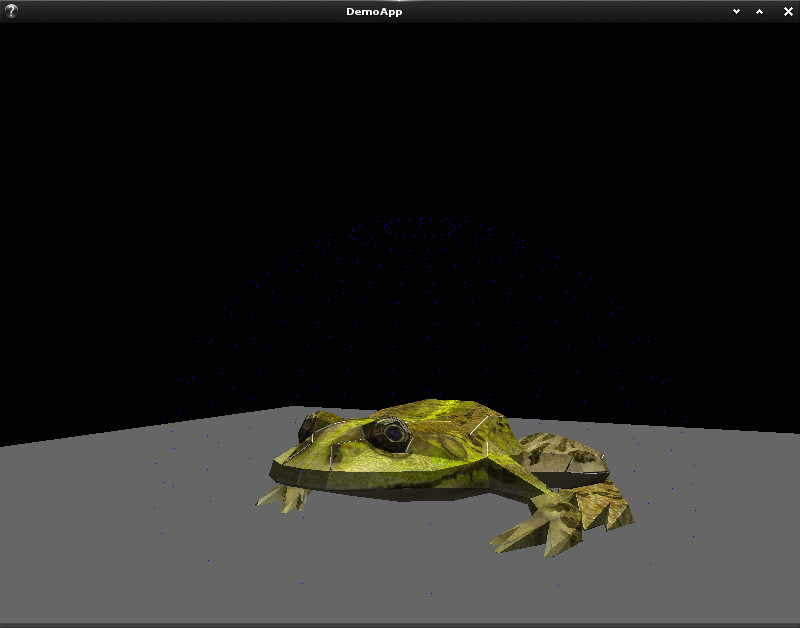
\includegraphics[scale=0.5]{images/z1.jpg}
\caption{Charakterystyki procesorów firmy Intel na przestrzeni 40 lat. Źródło: http://www.gotw.ca/}
\end{figure}

Aby zainicjować symulację należy użyć klawisza "t". Zostanie w ten sposób
stworzony model żaby, której model na licencji Royality Free
dostępny jest na stronie http://www.turbosquid.com/FullPreview/Index.cfm/ID/589370.

\begin{figure}[H]
\centering
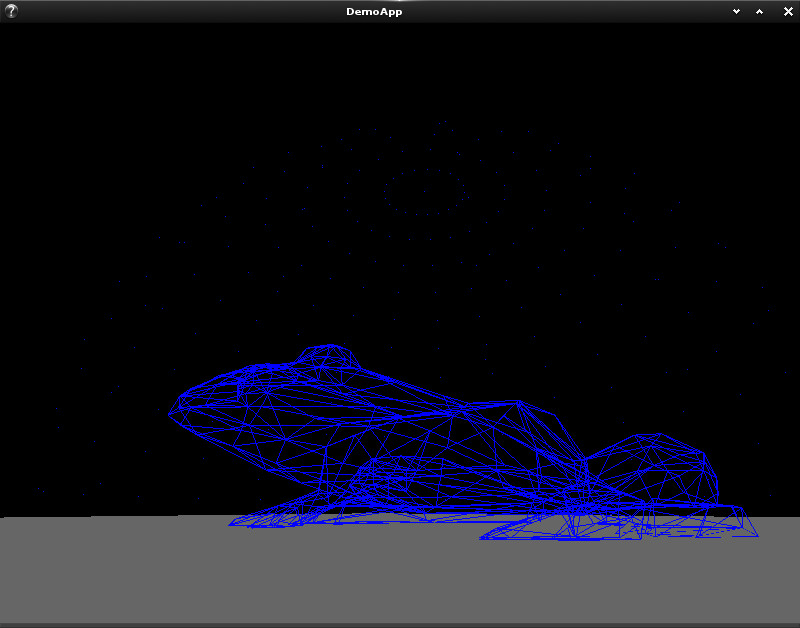
\includegraphics[scale=0.5]{images/z2.jpg}
\caption{Charakterystyki procesorów firmy Intel na przestrzeni 40 lat. Źródło: http://www.gotw.ca/}
\end{figure}

Program demonstracyjny posiada dwa tryby renderowania. W pierwszym wyświetlany
jest cały oteksturowany model wraz z oświetleniem, w drugim zaś renderowana jest
tylko siatka połączeń między wierzchołkami tworzącymi trójkąty. Aby przełączać
się między dwoma trybami należy użyć klawisza "m".

\begin{figure}[H]
\centering
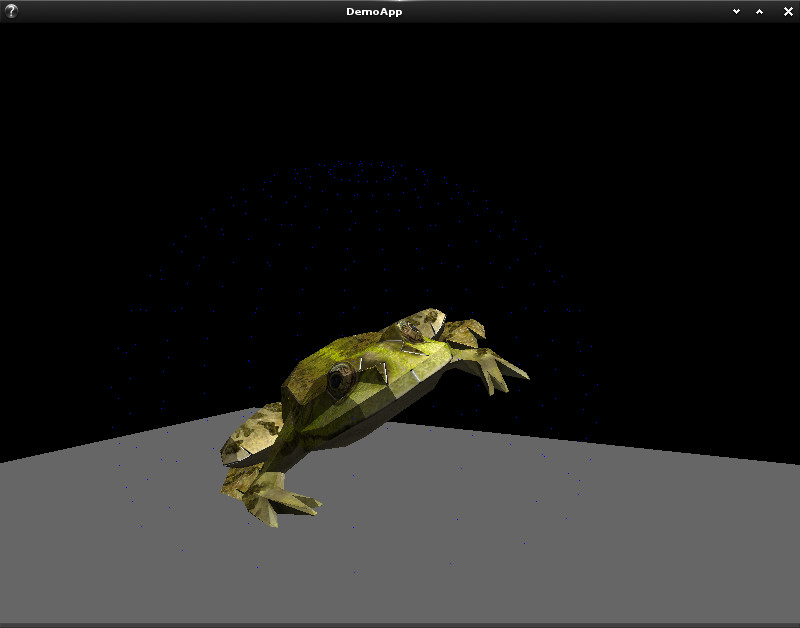
\includegraphics[scale=0.5]{images/z3.jpg}
\caption{Charakterystyki procesorów firmy Intel na przestrzeni 40 lat. Źródło: http://www.gotw.ca/}
\end{figure}

W stworzonej aplikacji istnieje możliwość interakcji z symulowanym ciałem
miękkim. W tym celu należy najechać myszą na obszar zajmowany przez model a
następnie nacisnąć i trzymać lewy przycisk myszy.

\begin{figure}[H]
\centering
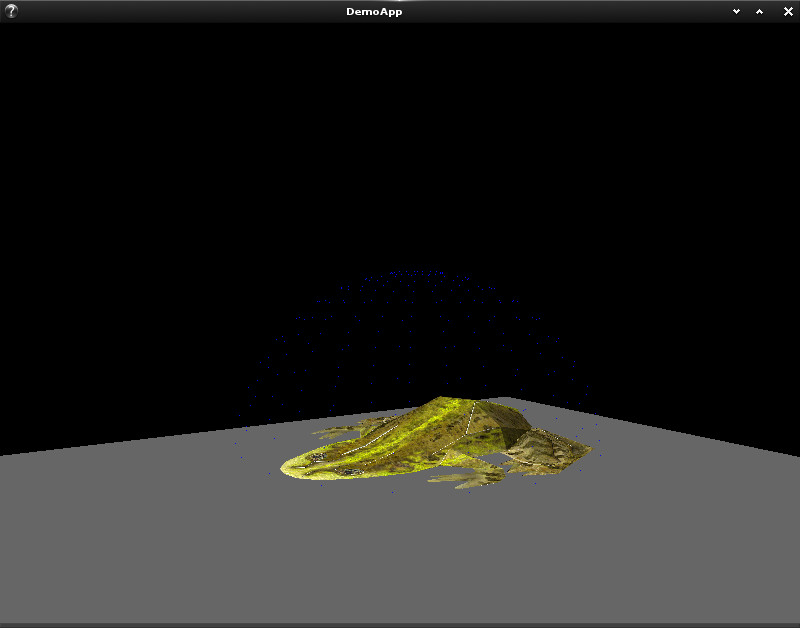
\includegraphics[scale=0.5]{images/z5.jpg}
\caption{Charakterystyki procesorów firmy Intel na przestrzeni 40 lat. Źródło: http://www.gotw.ca/}
\end{figure}

Możliwe jest również zmienianie współczynnika sprężystości symulowanego ciała. W
przypadku gdy jest on większy symulowane ciało zachowywać się będzie bardziej
jak bryła sztywna, natomiast dla małych wartości ciało wskazywać będzie zanik
wszelkich sił wewnętrznych. Zmiana sił sprężystości możliwa jest poprzez
klawisze '-' i '+'.

% GLWF
\subsection{Rysowanie okna}
W celu stworzenia okna aplikacji posłużono się open-sourcową biblioteką GLFW. Z
racji, że biblioteka te udostępnia interfejsy programisty napisane tylko w języku C
utworzona została klasa \texttt{GLFWApplication} opakowująca API biblioteki
GLFW (ang. wrapper). Oprócz zwykłego udostępniania metod, klasa ta spełnia
jeszcze dodatkowe funkcje. Udostępnia ona wirtualne metody \texttt{OnRender}
oraz \texttt{OnUpdate}, które będą wykorzystywane odpowiednio przy rysowaniu
ramki obrazu oraz przy symulacji fizyki. Dodatkowo klasa GLFWApplication rejestruje wszystkie błędy zgłaszane przez
GLFW i drukuje je do standardowego wyjścia błędów.

% statyczny krok symulacji
\subsection{Krok symulacji}
Kolejnymi funkcjonalnościami dostarczanymi przez klasę \texttt{GLFWApplication} jest
uruchomienie pętli głównej aplikacji oraz wywoływanie metod \texttt{OnUpdate} oraz \texttt{OnRender}.
Jest to niezbędne w celu zsynchronizowania odświeżania obrazu i
symulacji fizyki. Pętla główna zdefiniowana na listingu (\ref{main_loop})
pozwala na użycie stałego kroku czasu w symulacji fizyki przy jednoczesnym
zachowaniu możliwości odświeżania obrazu w różnej częstotliwości. Przyjęcie
stałego kroku czasu jest niezbędne w symulacji ponieważ
techniki w niej zaimplementowane są wrażliwe na jego zmianę, czego efektem jest
np. zmiana sztywności ciała obserwowana przy zmianie kroku czasu.

\begin{lstlisting}[caption=Pętla główna, label=main_loop]
void GLFWApplication::MainLoop(double delta)
{
	double accumulator = 0.0;
	lastFrameTime = glfwGetTime();

	while (!glfwWindowShouldClose(m_window)) {
		double currentTime = glfwGetTime();
		double frameTime = currentTime - lastFrameTime;

		if (frameTime > MAX_FRAME_TIME)
			frameTime = MAX_FRAME_TIME;

		accumulator += frameTime;
		lastFrameTime = currentTime;

		while (accumulator >= delta) {
			OnUpdate(delta);
			accumulator -= delta;
		}

		OnRender();
		glfwSwapBuffers(m_window);
		glfwPollEvents();
	}

	glfwDestroyWindow(m_window);
}
\end{lstlisting}

% łapanie obiektów
\subsection{Chwytanie obiektów}
W aplikacji demonstracyjnej możliwe jest ,,chwytanie'' części symulowanych
obiektów. Możliwe jest to dzięki funkcji z interfejsu programistycznemu
biblioteki (API). Jako parametry wejściowe funkcja ta przyjmuje półprostą (ang.
		Ray) oraz liczbę zmiennoprzecinkową oznaczającą maksymalną odległość
punktów od półprostej, które mają zostać ,,schwytane''. Operacja tworzenia
półprostej realizowana jest dwuetapowo. W pierwszym etapie ze współrzędnych
\texttt{x, y} myszki wyliczany jest odpowiadający im punkt w przestrzeni
trójwymiarowej, czyli tzw. współrzędnych świata (ang. world
		coordinates). Realizuje to funkcja \texttt{GetWorldCoordinates},
	zaimplementowana w klasie \texttt{Demo} dziedziczącej po klasie
	\texttt{GLFWApplication}. Jej implementacja
	przedstawiona jest na listingu poniżej:

\begin{lstlisting}[caption=Estymacja wektora w przstrzeni trójwymiarowej na
	podstawie pozycji myszki na ekranie, label=screen2world]
Ray Demo::GetRayFromCamera()
{
	glm::vec3 ret;
	glm::uvec2 mouse = GetMouseCoords();

	ret[0] = (2.0f * mouse[0]) / width - 1.0f;
	ret[1] = 1.0f - (2.0 * mouse[1]) / height;
	ret[2] = 0.0f;

	glm::vec4 pos = glm::vec4(ret, 1.0);
	pos = glm::inverse(renderer.GetProjectionMatrix()) * pos;

	pos[3] = 0.0f;

	pos = glm::inverse(mCamera.getCameraMatrix()) * pos;

	return Ray(mCamera.GetEyePosition(), pos.xyz());
}
\end{lstlisting}

Ideą funkcji przedstawionej na listingu \ref{screen2world} jest odwrócenie
procesu zachodzącego przy rysowaniu ramki obrazu przez bibliotekę OpenGL.
% dołożyć krótki schemat 
Na początku ze współrzędnych myszki tworzony jest trójwymiarowy wektor
wyrażony w tzw. znormalizowanych współrzędnych urządzenia (ang. Normalized
		Device Coordinates). Specyfikacja OpenGL zakłada, że współrzędne te zawierają się w
przedziale -1.0 do 1.0. Dodatkowo przy wyliczaniu drugiej współrzędnej
\texttt{ndc[1]} trzeba uwzględnić fakt, że biblioteka GLFW podaje współrzędne
myszki zaczynając od lewego górnego rogu okna, natomiast OpenGL zakłada, że
współrzędne (-1.0, -1.0) znajdują się w lewym dolnym rogu okna.

Trzecią koordynatą używaną w NDC jest wartość bufora głębokości. Może ona zostać
odczytana z bufora głębokości po wygenerowaniu ramki obrazu przy użyciu funkcji
OpenGL \texttt{glReadPixels}, jednak w przypadku gdy skonstruować chcemy tylko
półprostą każda wartość mieszcząca się przedziałach (-1, 1) będzie odpowiednia.
Kolejnym krokiem jest zamiana NDC do tzw. współrzędnych przycięcia (ang. clip
		coordinates). W tym celu musimy skonstruować czterowymiarowy wektor,
		 którego czwarta współrzędna jest współczynnikiem skalowania pozostałych
		 współrzędnych. Aby nie modyfikować wartości już wyliczonych
		 współrzędnych przyjmujemy że ostatnia współrzędna wektora jest równa 1.
		 
Kolejnym etapem jest odwrócenie wpływu macierzy projekcji. Dzieje się
poprzez przemnożenie wektora w współrzędnych przycięcia przez odwróconą
macierz projekcji. Ostatnim etapem jest odwrócenie wpływu macierzy
kamery, (jest ona odpowiednikiem macierzy OpenGL GLMODELVIEW).
Zanim jednak wektor zostanie przemnożony przez odwróconą macierz kamery,
	  ostatnia współrzędna $w$ wektora zostanie wyzerowana. Ma to za cel
	  wyeliminowanie translacji z przekształcenia, gdyż w ten sposób
	  otrzymalibyśmy finalną pozycję punktu we współrzędnych modelu.

\section{Biblioteka}
Biblioteka programistyczna jest najważniejszym i największym komponentem
stworzonym na potrzeby tej pracy. Implementuje ona metodę \texttt{Shape
	Matchingu} opisaną w rozdziale\ref{sec:shape}, wraz z jej modyfikacją wymienioną w
	podrozdziale \ref{ssec:region} oraz technikę zachowania
	objętości opisaną w rozdziale {\ref{sec:vol}.

Biblioteka napisana jest w języku C++ 

\begin{figure}[H]
\centering

\tikzset{
	  basic/.style  = {draw, text width=4cm, drop shadow, font=\sffamily,
		  rectangle},
		    root/.style   = {basic, rounded corners=2pt, thin, align=center,
				                   fill=green!30},
			  level 2/.style = {basic, rounded corners=6pt, thin,align=center,
				  fill=green!60,
				                     text width=8em},
			    level 3/.style = {basic, thin, align=left, fill=pink!60, text
					width=9.0em}
}
\begin{tikzpicture}[
  level 1/.style={sibling distance=55mm},
    edge from parent/.style={->,draw},
	  >=latex]

	  % root of the the initial tree, level 1
	  \node[root] {libsoftbody-engine}
	  % The first level, as children of the initial tree
	    child {node[level 2] (c1) {Fizyka}}
		  child {node[level 2] (c2) {Model}}
		    child {node[level 2] (c3) {Renderowanie}};

% The second level, relatively positioned nodes
\begin{scope}[every node/.style={level 3}]
\node [below of = c1, xshift=25pt] (c11) {CPUSoftBodySolver};
\node [below of = c11] (c12) {CUDASoftBodySolver};

\node [below of = c2, xshift=25pt] (c21) {SoftBody};
\node [below of = c21] (c22) {MeshData};
\node [below of = c22] (c23) {Material};
\node [below of = c23] (c24) {OBJParser};
\node [below of = c24] (c25) {OBJLexer};

\node [below of = c3, xshift=25pt] (c31) {Scene};
\node [below of = c31] (c32) {Shader};
\node [below of = c32] (c33) {VertexBuffer};
\node [below of = c33] (c34) {Camera};
\end{scope}

% lines from each level 1 node to every one of its "children"
\foreach \value in {1,2}
  \draw[->] (c1.192) |- (c1\value.west);

  \foreach \value in {1,...,5}
    \draw[->] (c2.192) |- (c2\value.west);

	\foreach \value in {1,...,4}
	  \draw[->] (c3.192) |- (c3\value.west);

\end{tikzpicture}

\caption{Stos CUDA. Źródło: Opracowanie własne.}
\label{cuda-model}
\end{figure}

\subsection{Model w formacie Wavefront}
% format obj - zalety w sb
% opis klas lekser i parser, mesh data
% opis formatu
% duplikowanie verteksów

\subsection{Renderowanie}
% opis klasy renderowania
% cienie i generacja normalnych

% stabilność numeryczna
\subsection{Solwer CPU}

\subsection{Solwer GPU}
 % opis klasy 
 % preprocessing
 % updatowanie verteksów
\subsection{Stabilność numeryczna}


\chapter{Optymalizacja}
\section{Benchmark}
\section{CPU}
\section{GPU}
\section{Porównanie}



\chapter{Zakończenie}





%\listoffigures
%\listoftables
%\listofcharts
%\listofdiagrams
%\listofcodes

%\appendix
%\chapter{Nazwa dodatku}

\nocite{*} 
\bibliographystyle{wfaiis}
\bibliography{literatura}

\end{document}
